
%%% Local Variables: 
%%% mode: latex
%%% TeX-master: "../lec02"
%%% End: 

\section{Introdução}

\begin{frame}
  \frametitle{``Máquina'' de von Neumann}
  \input{xx-vonneumann}
\end{frame}

\def\side{3cm}
\def\flabel#1{\scriptsize{#1}}
\begin{frame}
  \frametitle{Organização de um computador simples\footnote{\tiny Figura adaptada de Tanenbaum,2007, pg 29.}}

  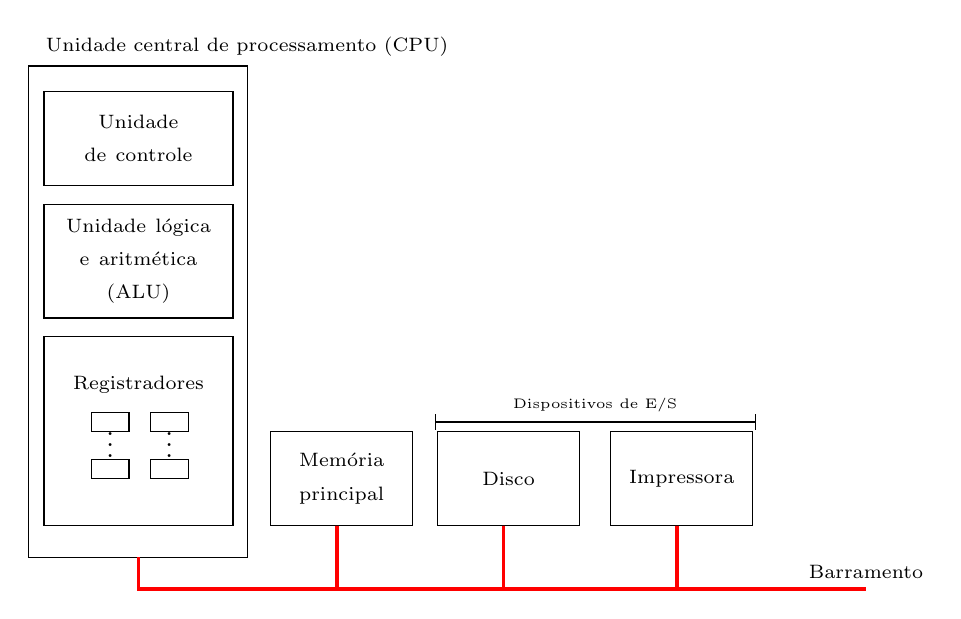
\begin{tikzpicture}[scale=0.8,
    boxtext/.style={text width=2cm,text centered, midway}
    ]
    %CPU
    \draw (0,0) rectangle +(\side,\side);
    \foreach \x / \y in {1/1,2.25/1,1/2,2.25/2} {
      \def\factor{0.25*\side}
      \draw (\factor*\x,\factor*\y) rectangle +(0.2*\side,0.1*\side);
      % draw vertical dots
      \ifnum\y=1%
      \node at (\factor*\x+0.1*\side,\factor*\y+0.22*\side) {$\vdots$};
      \fi
    }
    \node at (0.5*\side,0.75*\side) {\flabel{Registradores}};
    \draw (0,1.1*\side) rectangle +(\side,0.6*\side) 
    node[boxtext] {\flabel{Unidade l\'ogica e aritm\'etica (ALU)}};
    \draw (0,1.8*\side) rectangle +(\side,0.5*\side) 
    node[boxtext] {\flabel{Unidade de controle}};
    % cpu
    \draw (-0.25cm,-0.5cm) rectangle +(0.475cm+\side,2.6*\side)
    node[above] {\flabel{Unidade central de processamento (CPU)}};

    % dev
    \draw (1.2*\side,0) rectangle +(0.75*\side,0.5*\side) 
    node[boxtext] {\flabel{Mem\'oria principal}};
    
    % I/O
    \draw (0.25cm+2*\side,0) rectangle +(0.75*\side,0.5*\side) 
    node[boxtext] {\flabel{Disco}};
    \draw (3*\side,0) rectangle +(0.75*\side,0.5*\side) 
    node[boxtext] {\flabel{Impressora}};
    % I/O label
    \draw[|-|] (0.2cm+2*\side,0.55*\side) -- +(1.7*\side,0) 
    node[midway,above] {{\tiny Dispositivos de E/S}};


    % bus startx at cpu box
    \draw[draw=red,very thick] (0.5*\side,-0.5cm) to (0.5*\side,-1cm)
    to (1.55*\side,-1cm) to (1.55*\side,0)
    to (1.55*\side,-1cm) to (0.25cm+2.35*\side,-1cm)
    to (0.25cm+2.35*\side,0) to (0.25cm+2.35*\side,-1cm)
    to (3.35*\side,-1cm) to (3.35*\side,0)
    to (3.35*\side,-1cm) to (4.35*\side,-1cm) node[above] {\flabel{Barramento}};

    %% becomes noise
    %%\node[text width=3cm] at (4*\side,1.75*\side) {\flabel{1 CPU + 2 dispositivos de entrada e saída}};
  \end{tikzpicture}
  
\end{frame}


\def\sectiontitle{Operações do hardware do computador}

\begin{frame}{\sectiontitle}
  
\begin{block}{Operações básicas}
  \begin{itemize}
  \item Aritmética
    \begin{itemize}
    \item Adição,
    \item Subtração,
    \item Multiplicação,...
    \end{itemize}
  \item Manipulação de dados - modelo {\em load$\slash$store}
    \begin{itemize}
    \item Carga ({\em load});
    \item Armazenamento ({\em store}). 
    \end{itemize}
  \end{itemize}
\end{block}
\end{frame}

\begin{frame}{Linguagem de montagem ({\em assembly})}
  
  \begin{block}{Arquitetura MIPS? Por quê?}
    \begin{itemize}
    \item Conjunto reduzido de instruções favorecendo simplicidade;
    \item Maior quantidade de registradores quando comparada com
      outras arquiteturas;
    \item Utilização de arquiteturas semelhantes em grande escala
      (SPARC, ARM, PowerPC,...);
    \item Simuladores disponíveis para aprendizado.
    \end{itemize}
  \end{block}
\end{frame}

\begin{frame}{Sequência de geração de código binário}
  
\input{img/000_translation_hierarchy_C}

\end{frame}

\begin{frame}{Alocação de memória feita pelo carregador ({\em linker})}
  
\begin{center}
\input{img/000_memory_allocation}
\end{center}

\end{frame}


\section{Operações aritméticas}

\begin{frame}[fragile]{Compilando C para MIPS}
$\Rightarrow$ compilador\\

a $\leftarrow$ \$s0, {\color{blue} b $\leftarrow$ \$s1}, 
{\color{red}c $\leftarrow$ \$s2}, { d
  $\leftarrow$ \$s3},
{ \color{green!50!black!90!}  e $\leftarrow$ \$s4}\\

\bigskip
  \begin{minipage}[h]{0.275\linewidth}
    \begin{tabbing}
      a \= $=$ \= {\color{blue}b} \= $+$ \= {\color{red}c}; $\Rightarrow$\\
      d \> $=$ \> a \> $-$ \> {\color{green!50!black!90!}e}; $\Rightarrow$\\
    \end{tabbing}
  \end{minipage}
  \only<2->{
  \begin{minipage}[h]{0.7\linewidth}
    \small
    \begin{tt}
      {\bf add} \$s0,{\color{blue}\$s1},{\color{red}\$s2} {\color{gray}\footnotesize \# registro \$s0 recebe b + c}\\
      {\bf sub} \$s3,\$s0,{\color{green!50!black!90!}\$s4} {\color{gray}\footnotesize \# registro \$s3 recebe a - e}\\
    \end{tt}
  \end{minipage}
}

\bigskip

\small
\only<3->{
Como um compilador poderia converter a seguinte atribuição em C?\\
\begin{tt}
  \begin{tabbing}
expressão:    \=f  = (\=g + \=h) - (\=i + \=j);\\
    \>| \>| \>| \>| \>|\\
registros:    \>\$s0 \>\$s1 \>\$s2 \>\$s3 \>\$s4
  \end{tabbing}
\end{tt}
}

\only<4->{
\begin{tt}
  {\bf add} \$t0,\$s1,\$s2 {\color{gray}\footnotesize \# registro \$t0 recebe g + h}\\
  {\bf add} \$t1,\$s3,\$s4 {\color{gray}\footnotesize \# registro \$t1
    recebe i + j}\\
  {\bf sub} \$s0,\$t0,\$t1 {\color{gray}\footnotesize \# f recebe \$t0 -
    \$t1 $\equiv$ (g + h) - (i + j)}\\
\end{tt}
}
\end{frame}


\begin{frame}[fragile]{Operações aritméticas com constantes}
$\Rightarrow$ compilador\\

a $\leftarrow$ \$s0, {\color{blue} b $\leftarrow$ \$s1}, 
c $\leftarrow$ \$s2\\

\bigskip
  \begin{minipage}[h]{0.275\linewidth}
    \begin{tabbing}
      a \= $=$ \= {\color{blue}b} \= $+$ \= {\color{red}20}; $\Rightarrow$\\
      c \> $=$ \> a \> $-$ \> {\color{green!50!black!90!}8}; $\Rightarrow$\\
    \end{tabbing}
  \end{minipage}
  \only<2->{
  \begin{minipage}[h]{0.7\linewidth}
    \small
    \begin{tt}
      {\bf addi} \$s0,{\color{blue}\$s1},{\color{red}20} {\color{gray}\footnotesize \# registro \$s0 recebe b + 20}\\
      {\bf subi} \$s2,\$s0,{\color{green!50!black!90!}-8} {\color{gray}\footnotesize \# registro \$s3 recebe a - 8}\\
    \end{tt}
  \end{minipage}
}

\bigskip
-- Inicialização\\
\only<3->{
  \begin{minipage}[h]{0.275\linewidth}
    \begin{tabbing}
      a \= $=$ \= {\color{blue}0}; $\Rightarrow$\\
    \end{tabbing}
  \end{minipage}
}
\only<4->{
  \begin{minipage}[h]{0.7\linewidth}
    \small
    \begin{tt}
      {\bf move} \$s0,\$zero {\color{gray}\footnotesize \# \$s0
        recebe o valor zero}\\
    \end{tt}
  \end{minipage}
}
\end{frame}

\section{Exercícios I}

\begin{frame}{Exercícios I}
  \begin{itemize}

  \item Operações aritméticas
    \begin{enumerate}
    \item $f = g + (j + 2)$
    \item $f=f+g+h+i+j+2$
    \item $f=g- (f - 5)$
    \end{enumerate}
    \bigskip
  \end{itemize}
  
\end{frame}
